\subsection*{Life-cycle state machines}
In this section we show the important life-cycle state machines, alogn with a small explanation of them.
\subsubsection*{Express Lane Check-in}
The ‘Express Check-in Toll Lane’-component, seen in \autoref{fig:life_cycle_statemachine_toll_lane_computer_express_check_in}, receives a message from the antenna to indicate that a vehicle with a toll tag has entered the lane. It reacts by sending a message to the station server to check that the tag is valid. If it receives true it tells the station server to check in the tag, opens the barrier, then closes it when the antenna informs it that the tag can no longer be detected.  Otherwise it goes to a faulty tag state and waits for a cashier to resolve the situation. 
\begin{figure}[H]
\centering
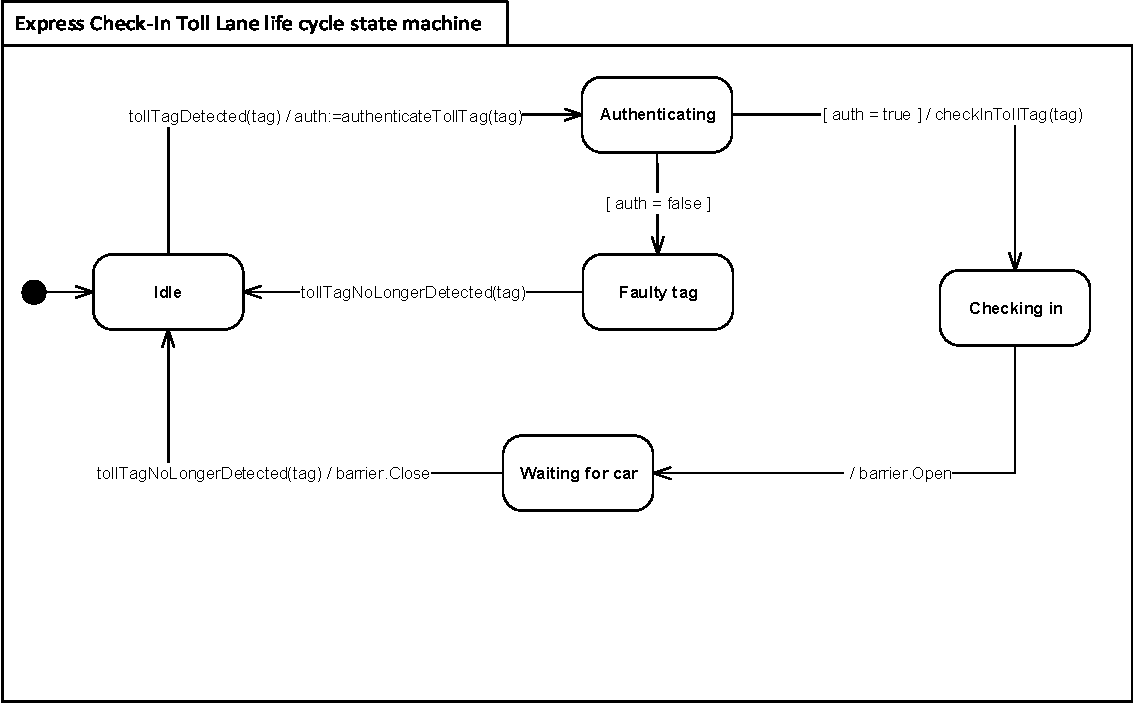
\includegraphics[width=0.7\linewidth]{img/protocol_state_machine/life_cycle_statemachine_toll_lane_computer_express_check_in.png}
\caption{The life-cycle state machine for express lane check-in}
\label{fig:life_cycle_statemachine_toll_lane_computer_express_check_in}
\end{figure}

\subsubsection*{Express Lane Check-out}
The ‘Express Check-out Toll Lane’-component, seen in \autoref{fig:life_cycle_statemachine_toll_lane_computer_express_check_out}, receives a message from the antenna to indicate that a vehicle with a toll tag has entered the lane. It reacts by sending a message to the station server to check that the tag is checked in. If it receives true it tells the station server to check out the tag, opens the barrier, then closes it when the antenna informs it that the tag can no longer be detected.  Otherwise it goes to a faulty tag state and waits for a cashier to resolve the situation. 
\begin{figure}[H]
\centering
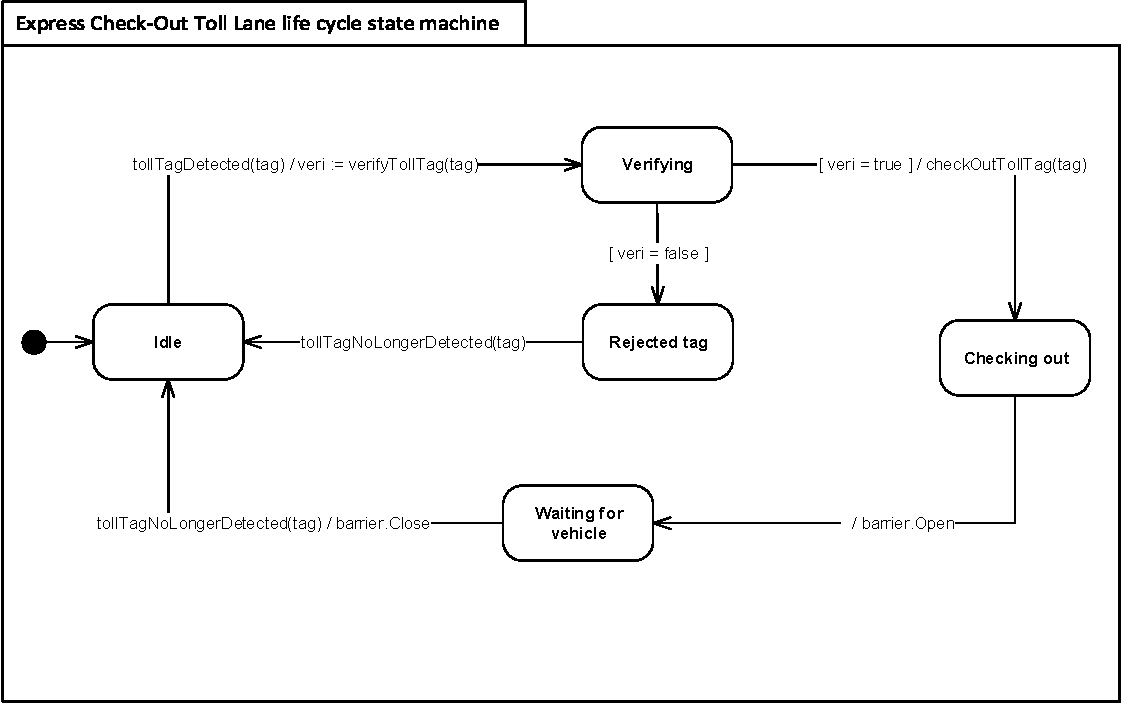
\includegraphics[width=0.7\linewidth]{img/protocol_state_machine/life_cycle_statemachine_toll_lane_computer_express_check_out.png}
\caption{The life-cycle state machine for express lane check-out}
\label{fig:life_cycle_statemachine_toll_lane_computer_express_check_out}
\end{figure}

\subsubsection*{Normal Lane Check-in}
The ‘Normal Check-in Toll Lane’-component, seen in \autoref{fig:life_cycle_state_machine_toll_lane_computer}, waits for the touch screen to send information about a vehicle. It returns the price for that vehicle, then waits to receive payment via cash or credit card. If payment is received via card, it contacts the bank about the transaction. It then prints a ticket and opens the barrier long enough for the customer to pass.
\begin{figure}[H]
\centering
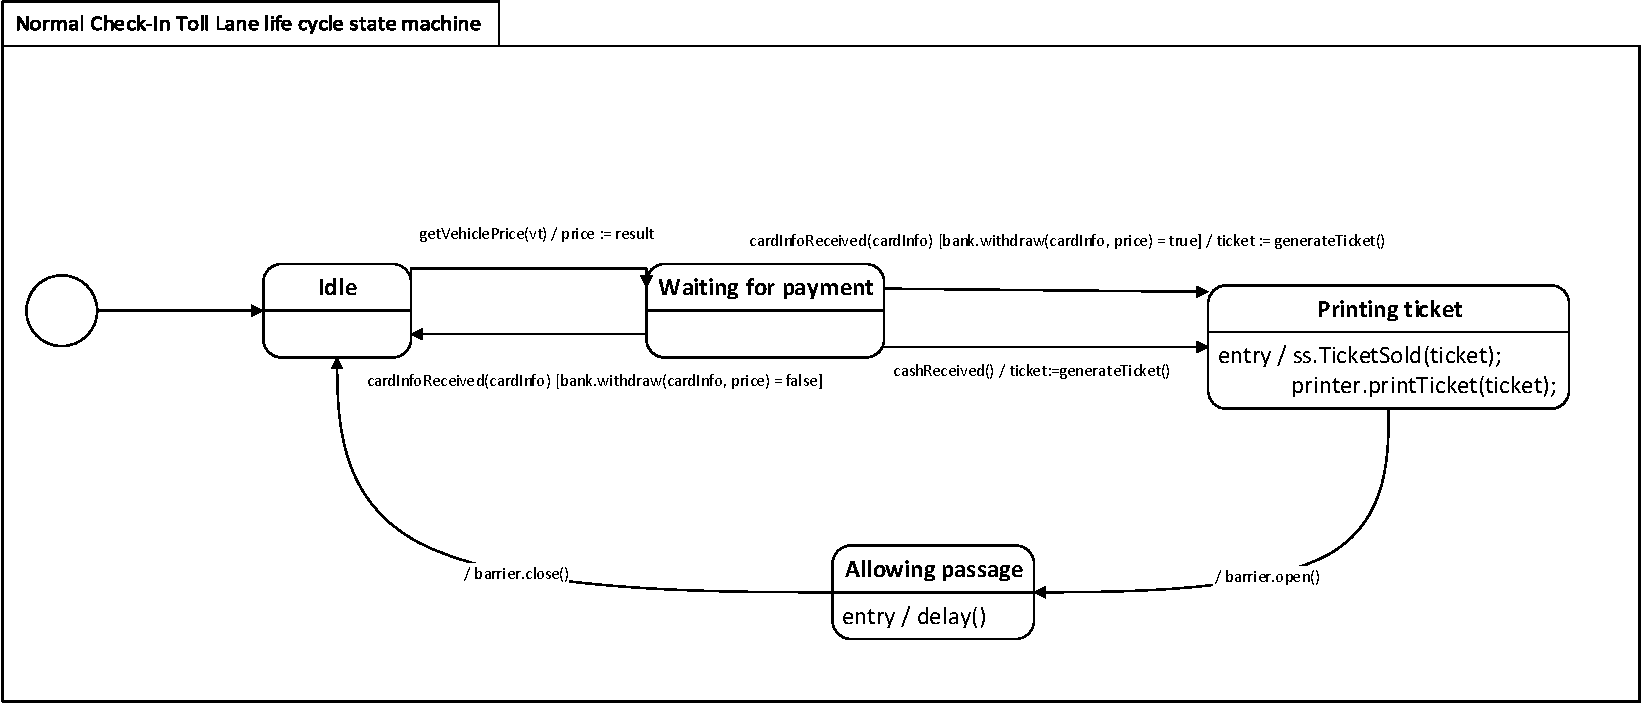
\includegraphics[width=0.7\linewidth]{img/protocol_state_machine/life_cycle_state_machine_toll_lane_computer.png}
\caption{The life-cycle state machine for normal lane check-in}
\label{fig:life_cycle_state_machine_toll_lane_computer}
\end{figure}

\subsubsection*{Normal Lane Check-out}
The ‘Normal Check-out Toll Lane’-component, seen in \autoref{fig:life_cycle_state_machine_toll_computer_normal_lane}, waits for a ticket to be inserted. When it is, it contacts the station server to validate the ticket. If the ticket is valid, it opens the barrier, waits for the customer to leave, then closes the barrier. Otherwise it goes to an invalid ticket state and waits for a cashier to resolve the situation.
\begin{figure}[H]
\centering
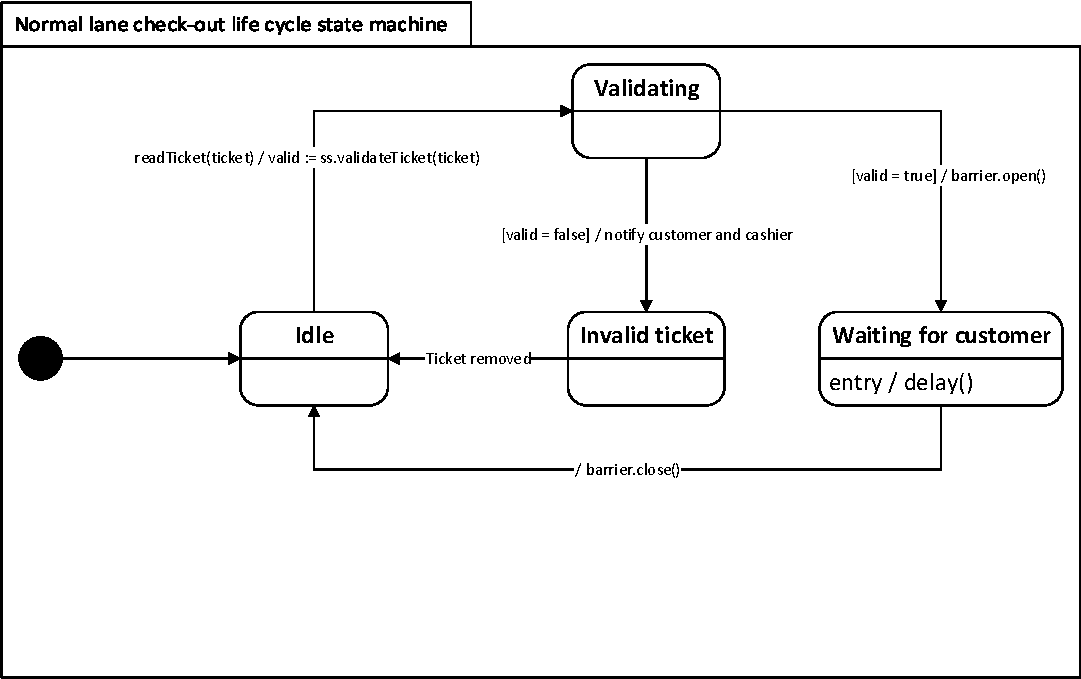
\includegraphics[width=0.7\linewidth]{img/protocol_state_machine/life_cycle_state_machine_toll_computer_normal_lane.png}
\caption{The life-cycle state machine for express lane check-out}
\label{fig:life_cycle_state_machine_toll_computer_normal_lane}
\end{figure}

\subsubsection*{Station server}
The ‘Station server’-component, seen in \autoref{fig:life_cycle_state_machine_station_server}, sends messages between the Toll Lane and the Enterprise Server.
\begin{figure}[H]
\centering
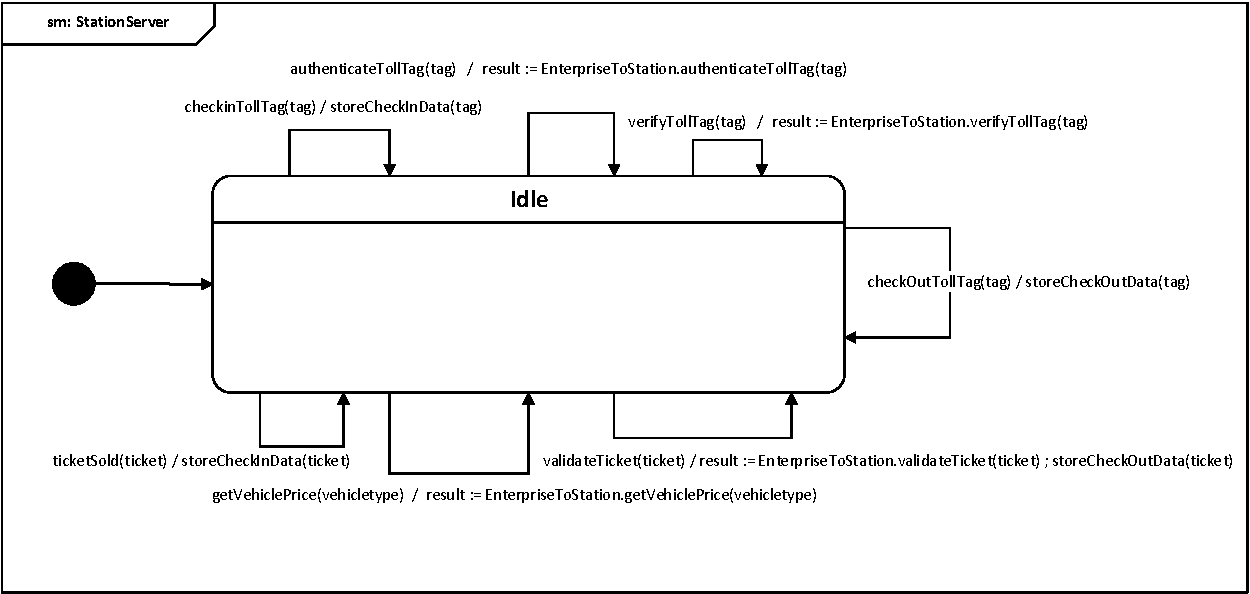
\includegraphics[width=0.7\linewidth]{img/protocol_state_machine/life_cycle_state_machine_station_server.png}
\caption{The life-cycle state machine for express lane check-out}
\label{fig:life_cycle_state_machine_station_server}
\end{figure}


\subsubsection*{Enterprise server}
As the inner workings of the enterprise server is quite complex we have split up the it's functionality into multiple diagrams to keep it simple to understand. Each diagram show the same concurrent state \texttt{Working}. That means all parts of all the diagrams are running concurrently. In the following we will go into detail into each diagram and go through each part of those diagrams.

\paragraph*{Part 1} In \autoref{fig:life_cycle_state_machine_enterprise_server} we first show the part which handles customers buying toll tags online through the webserver. The customer fills out the form, and if his bank informations can be validated we store his data and places the order for the toll tag.

Next we show the simple interaction when compiling reports for the enterprise manager.

Finally we show how the enterprise servers authenticates toll tags. First we authenticate, and then check if the toll tag is expired.

\begin{figure}[H]
\centering
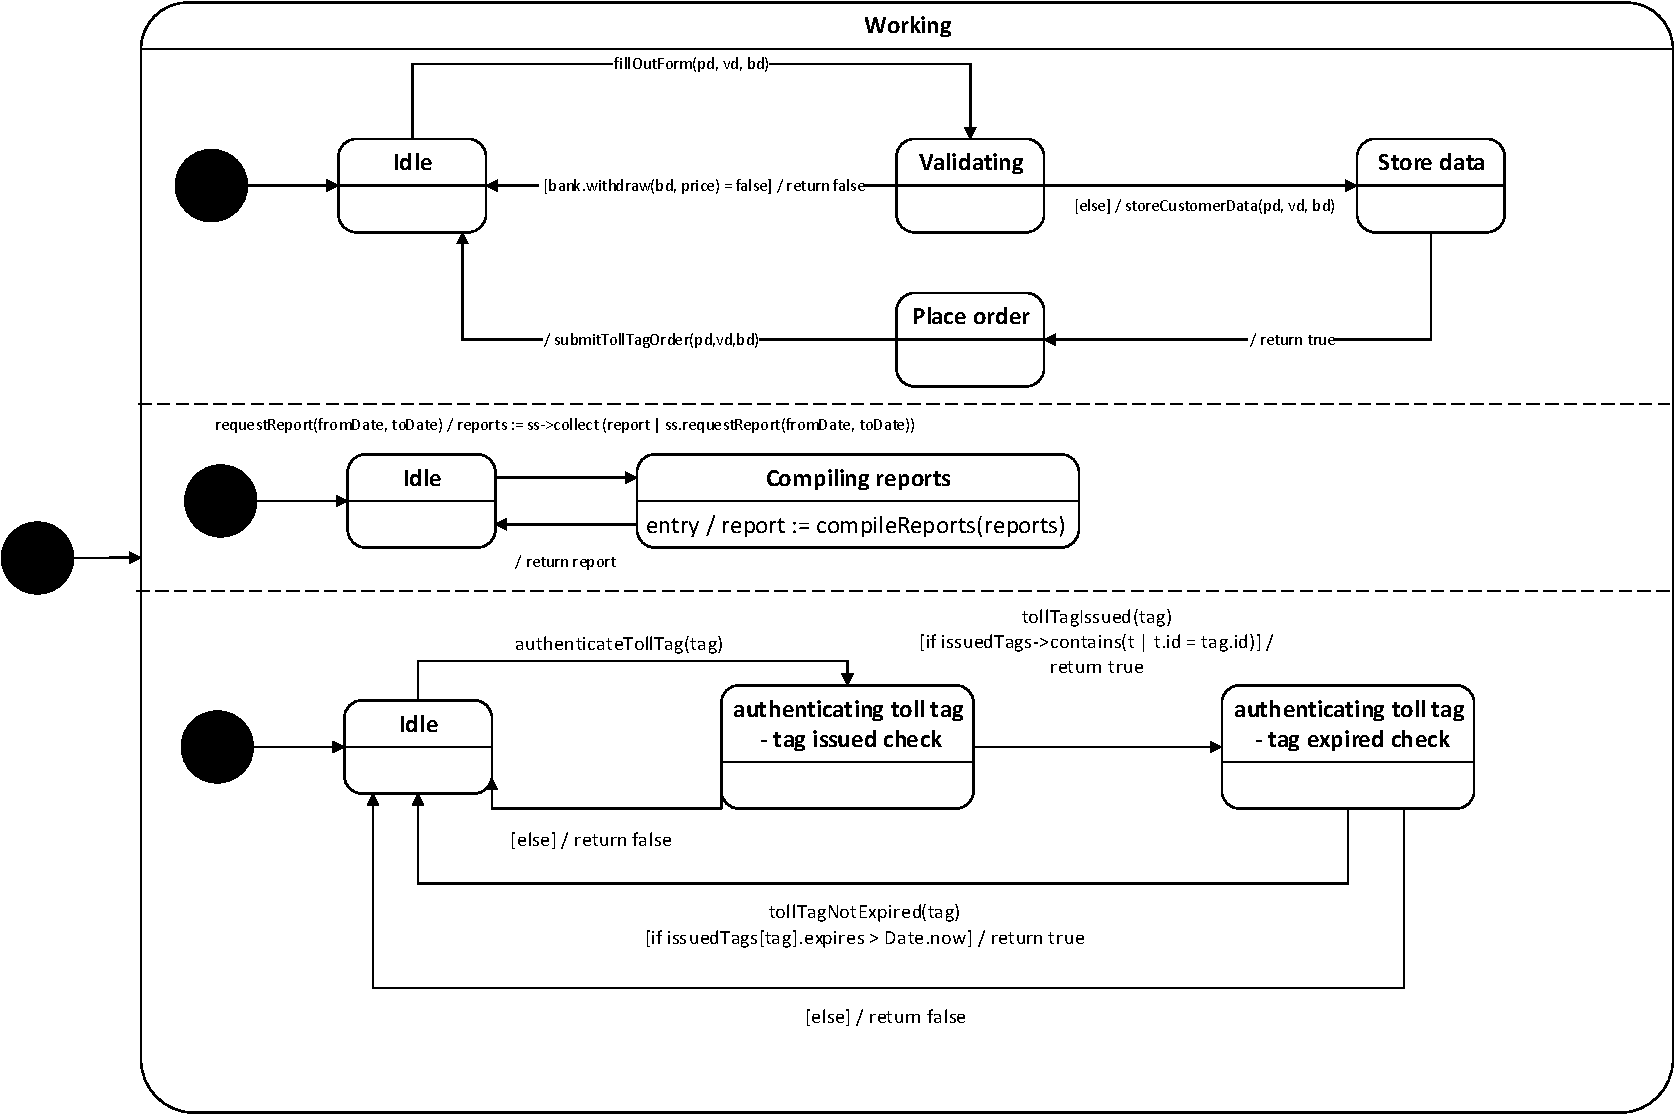
\includegraphics[width=0.7\linewidth]{img/protocol_state_machine/life_cycle_state_machine_enterprise_server.png}
\caption{The life-cycle state machine for express lane check-out}
\label{fig:life_cycle_state_machine_enterprise_server}
\end{figure}

\paragraph*{Part 2} In \autoref{fig:life_cycle_state_machine_enterprise_server_part2} we show how the enterprise server handles check-in and check-out with a toll tag. For checking in we register the relevant information to be used for reports and for checking out again. \textit{\textbf{\underline{REVIEW THIS AFTER LOOKING AT DIAGRAM}}}

\begin{figure}[H]
\centering
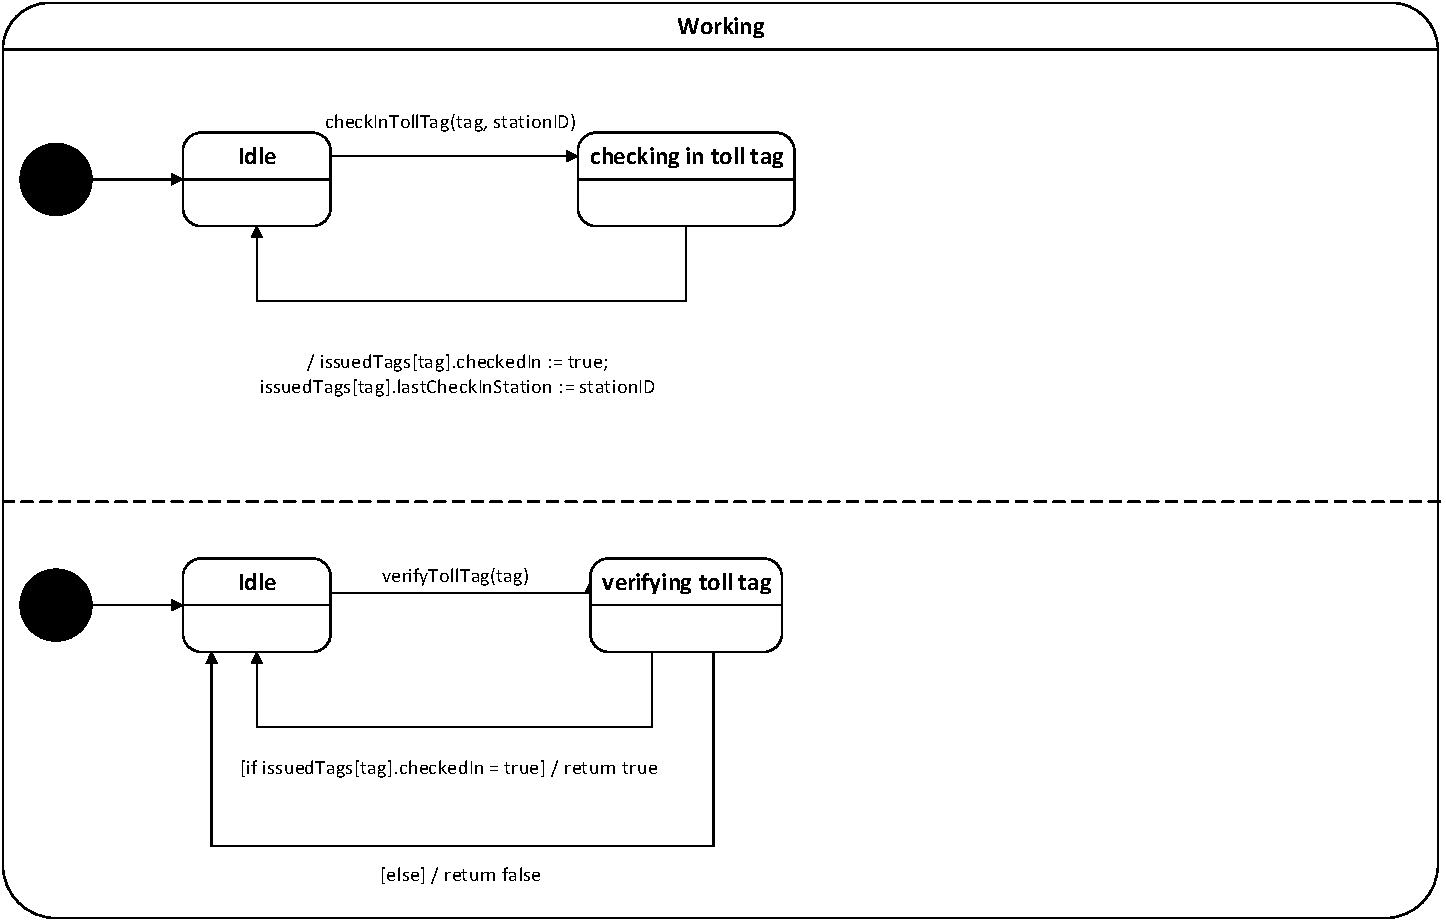
\includegraphics[width=0.7\linewidth]{img/protocol_state_machine/life_cycle_state_machine_enterprise_server_part2.png}
\caption{The life-cycle state machine for express lane check-out}
\label{fig:life_cycle_state_machine_enterprise_server_part2}
\end{figure}

\paragraph*{Part 3} In \autoref{fig:life_cycle_state_machine_enterprise_server_part3} .

\begin{figure}[H]
\centering
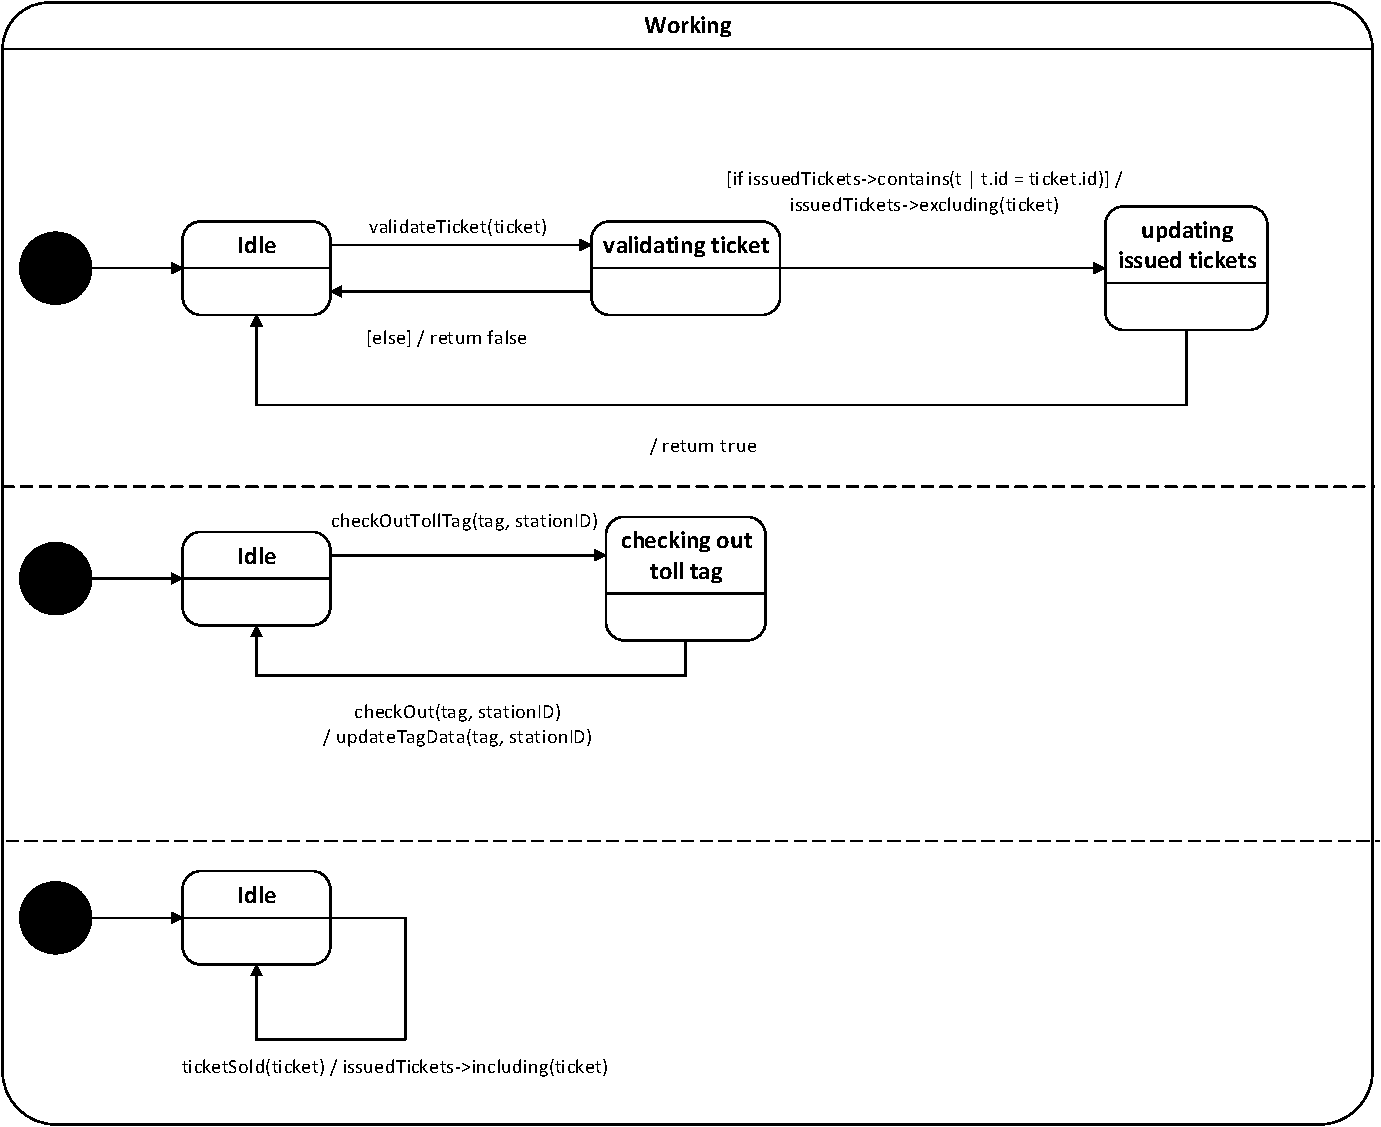
\includegraphics[width=0.7\linewidth]{img/protocol_state_machine/life_cycle_state_machine_enterprise_server_part3.png}
\caption{The life-cycle state machine for express lane check-out}
\label{fig:life_cycle_state_machine_enterprise_server_part3}
\end{figure}